\chapter {Functional requirements}

The functional requirements are based on the non-functional requirements and aim to realize those. Additional requirements are derived from the technical environment and its specifications. \\
To be able to display the data of Wikidata, ArticlePlaceholder needs to be based on Wikibase and MediaWiki.
As MediaWiki is written in PHP, the main part of the extension needs to make use of that language as well as the services provided by MediaWiki and Wikibase. \\
The programming language for scripts on Wikipedia is Lua. Therefore the parts that will be user-editable need to be written in Lua. This way they can be overwritten by the local communities. \\
The default for the content pages presents the information and data in a useful way, and to make it visually appealing, should make use of images when possible.
For users without access to a computer (as in the Scenario of Edha) the layout of the extension is required to be responsive and work on mobile devices. \\
The following requirements are not necessarily all in the scope of this thesis but describe the finished ArticlePlaceholder extension as it would be deployed to Wikipedia.

\section{Naming}
Since the users need to find the ArticlePlaceholder easily it is implemented as a SpecialPage. This SpecialPage should have a short name that is easy to remember. \todo{just remove the sentence!?}\st{Calling the special page ``ArticlePlaceholder'' would be confusing due to people expecting it to generate a whole article in that case.}  Therefore it is called ``AboutTopic''.

\section{Display ArticlePlaceholder}
The pages displaying the content of a Wikidata item focus on a clear differentiation between the layout of the placeholder and what a user-written article would look like. They still contain elements of the well-known Wikipedia layout to appeal to readers and fit in with the other content. \\
There must be a default layout but it is very important to give the user control over everything and therefore let every part be user editable for users as Julian who want to adjust the layout to their communities' needs.

\section{Internationalization}
It is important to have the whole extension offer the possibility to be localized from the beginning. This is necessary for the extension to be used by an international community. \\ 
``Internationalization refers to the adaptation of products to support or enable localization for international markets. Key features of internationalization have always been the support of international natural language character sets, separation of locale-specific features such as translatable strings from the software code base and the addition of functionality or features specific to foreign markets. Without internationalization, localizing a product can be very challenging'' states \citet[23]{localization}. \\
Since the data on Wikidata is multilingual, this focuses more on aspects like labels on buttons and the name of the special page itself.

\section{Discover ArticlePlaceholder}

There are multiple ways for a reader to get to an ArticlePlaceholder. 

\subsection{SpecialPage URL}
Beside the input form there should be a way to directly link to an ArticlePlaceholder page as necessary for the scenario of Heather.

\subsection{Search}
To be able to discover an ArticlePlaceholder while looking for a topic the generated pages are added to the search on Wikipedia. There are different places for the results in the search page. They could be attached to the bottom of the results or placed to the right of the regular search results. \\
\\
It is important to remark, that the notability criterias on a Wikipedia are not necessarily the same as on Wikidata. The results in the search should be limited to notable items. \\
Showing only notable items is especially important since article creation should only be encouraged when it makes sense in order to not have articles created, that would be deleted by other users. That would hurt the community building and trust the ArticlePlaceholer is supposed to be working on. \\
Since it is hard to decide, which content is actually notable, the items appearing in the search should be limited to only the ones having at least two to three statements and two sitelinks to the same project (like Wikipedia or Wikivoyage). \\
\\
Catrin's scenario showed how a user would start their research with an ArticlePlaceholder. Therefore wherever possible the ArticlePlaceholder should link to existing Wikipedia articles. There is not yet an easy solution to get the data from Wikidata in a form making it easy to link it. Therefore this is not in the scope of this thesis.
\\
A lot of users will research information on web search engines such as Google and get to Wikipedia from the results. To make the data provided by the ArticlePlaceholder accessible for those users it will be necessary to have them the generated pages indexable. \todo{numbers}
\begin{figure}[H]\label{fig:CircleSearch}
	\centering
	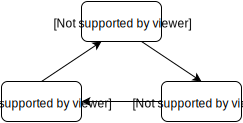
\includegraphics[width=80mm]{diagrams/CircleSearchAttention.png}
	\caption{Problem for small Wikipedias}
	\label{diagramCircleSearch}
\end{figure}
As described in figure~\ref{fig:CircleSearch} a problem of the small Wikipedia projects is being stuck in a vicious circle: Since they have few articles, they do not get a lot of attention via search engines such as Google, so they are not able to find new editors and therefore they do not have a lot of articles. \\
\\
Making ArticlePlaceholder accessible for search engines is outside the scope of this thesis but will be an important point in the following development of the extension. 

\subsection{Red links}
\todo[inline]{Requirements klarer machen}
\begin{quotation}
A red link (...) signifies a link to a page that is either non-existent or deleted. 
\end{quotation} \citep{wiki:01}

Red links are used a lot in Wikipedia to indicate an article, which is not there but should exist. Today it leads the user to an empty \textit{"create article"} page. In the future it should rather bring them to an ArticlePlaceholder, which offers them the option to create an article. Due to the high technical complexity of matching the titles of the red links to the Wikidata items, this topic is out of the scope for this thesis but will be an important part of the future development of the ArticlePlaceholder extension. There is a discussion on realizing so called \textit{smart red links} however, which is an approach for this issue and is discussed in the section~\ref{sec:redLinks}: \nameref{sec:redLinks}.

\section{Creation of an article from the ArticlePlacehoder}
Starting at the ArticlePlaceholder created by the extension the user might want to create an article to provide more information and give this data a context, that only natural language can provide. \\
There are two options to do so which are considered for now: Creating an article from scratch or translating an existing article into the user's language. \\
The challenge is to encourage editors to add a new article if appropriate and at the same time prevent vandalism, which is, according to \citet{wiki:33}, `` is any addition, removal, or change of content, in a deliberate attempt to damage Wikipedia. Examples of typical vandalism are adding irrelevant obscenities and crude humor to a page, illegitimately blanking pages, and inserting obvious nonsense into a page. Abusive creation or usage of user accounts and IP addresses may also constitute vandalism.'' \\ 
The title for the article they want to create might differ from the label of the item due to the local Wikipedia's rules and customs. Therefore a user must be able to enter a title for the page that does not exist on that Wikipedia yet. \\
After entering the title of the new article, the user is redirected to an empty editing page, where they can add their content. \\
In the future, it is intended to add the data provided by Wikidata to the editing page so the user can use it while writing the article. 

\subsection{Content translation}
Using the content translation tool\footnote{\href{https://www.mediawiki.org/wiki/Content_translation}{Content translation tool}}, the user should be able to translate the article from an existing article in another language. This is not in the scope of this thesis, the focus for now is to create articles from scratch. \\

\section{Ordering of statement groups}
The data in Wikidata is not ordered in a meaningful way. The ArticlePlaceholder is aimed at readers, who want to get an overview of the topic and therefore only need the most important data on a topic and should not be overwhelmed with everything available. \\
\\
To keep the control with the editors, there should be a list of properties maintained on-wiki. They are ordered by their importance. \\
The ordered list includes labels of the properties as well as their numbers for user not familiar with Wikidata. The list can be annotated with comments on each line to add additional information and help other editors understand the context of the property and its place in the ordered page. \\
This list is only editable by administrators on the Wikipedia to reduce constant changing of information displayed. \\
This list is then used to order and filter the statements on each ArticlePlaceholder page. 

\section {Identifier}
For the reader to be able to handily look up more information on other sites beside Wikimedia projects they need to be distinguishable from the other statements and always show up on the ArticlePlaceholder. \\
\\
Identifier differ from the other properties not only in their distinguished placement in the layout but also thematically. They are IDs used for the entity in other ontologies. Therefore they should not be included in the list of ordered statements. \\
There was not a data type for identifier in Wikidata while the extension was developed but it is introduce and deployed now. \\
Until the data type was deployed, it was sufficient to have a static list of property IDs in the extension. This list includes all identifiers used in Wikidata and can be exchanged later on with the proper handling of all statements with the identifier data type.

\section{Caching}
Since the generated content pages will be accessed frequently \todo{numbers: WP page views per day} it will be necessary to implement some form of caching for them. With caching it would be possible to limit the amount of requests to Wikidata services, too, which will show an improvement in the performance. This is not part of this thesis however.

\section {Unit tests}
Especially the main code in PHP should be covered completely by unit tests. \\
It is necessary to set up continues integration in a way that it is integrated with MediaWiki and Wikibase to make the code not only conform to coding conventions but also to run the unit test automatically. This will reduce the time spent with code reviews, testing and bug fixing. \\
This is not part of this thesis but is done in cooperation with the Wikidata team while working on the extension. Neither are the integration tests and tests for the Lua code in the scope of this thesis. \\ 